\section{A stylized model of sovereign default with robustness \label{sec:2permodel}}

This section presents a stylized sovereign default model to conceptually explore the interaction between state-contingent debt and robustness. A small open economy, populated by a government and a representative agent, faces risk-neutral competitive foreign lenders. The world lasts for two periods in which the government receives endowments $(y_1, y_2)>0$. There is uncertainty about $z$ which determines the value of income in the second period $y_2(z)$.

\paragraph{Assets} Only one type of security is traded.\footnote{In line with previous studies \citep{BorenszteinMauro2004, Durdu, HMindexed2012, HMSP16, SandlerisSaprizaTaddei2017, KimOstry2021, SosaPadillaStruzenegger2021}, we abstract from the portfolio problem and compare the cases of noncontingent and contingent debt.}
When the government issues debt, it promises a repayment $R(z)$ in state $z$ of the second period. Different specifications of the stipulated repayment function $R$ represent different types of state-contingent debt structures. We focus on four different types of repayment functions summarized in Table \ref{tab:R(z)}.

\begin{table}[!hbtp]\centering \small
\caption{Stipulated repayment functions}\label{tab:R(z)}
\begin{tabular}{@{}lccc@{}}\toprule
  \textbf{Type of debt} & \multicolumn{3}{c}{\textbf{Stipulated repayment}} \\\midrule
  Noncontingent debt & $R(z)$ & $ = $ & $1$ \\
  Linear indexing & $R^\alpha(z)$ & $ = $ & $1 + \alpha \left( y_2(z) - \mathbb{E}_1\left[y_2(z)\right] \right) $ \\
  Threshold debt & $R^\tau(z)$ & $ = $ & $\ind\left(y_2(z) > \tau\right)$ \\
  Optimal design & $R^\star(z; \theta)$&       & {\footnotesize chosen state by state}\\\bottomrule
\end{tabular}
\end{table}
Noncontingent debt promises a constant repayment regardless of the state, while the repayment of linearly-indexed debt depends on the difference between realized output and its mean, with a slope parameter of $\alpha \geq 0$.\footnote{In the model, we use $\max\{0,R^\alpha(z)\}$ when considering linearly-indexed debt to keep repayments nonnegative. We skip the $\max$ in the description to keep the notation succint.} Threshold debt pays only if the state is above a minimum level. Finally, we compute the debt structure that maximizes the utility of the government by promising non-negative repayments $R^\star$ state-by-state in a flexible manner. Our notation anticipates that the optimal design depends on the lenders' preferences as summarized by the robustness parameter $\theta$ introduced below.

\paragraph{Government} The government is benevolent and makes decisions on a sequential basis. The government acting in period $j \in \{1,2\}$ maximizes $\mathbb{E} \left[ \sum_{t=j}^2 \beta_b^{t-j} u\left( c_t \right)\right]$, where $\mathbb{E}$ denotes the expectation operator, $\beta_b \in (0,1]$ is the government's discount factor, $c_{t}$ represents period-$t$ consumption in the economy, and the utility function $u$ is increasing and concave. The government borrows to finance consumption in period 1, taking as given the stipulated repayment function $R$. The government may choose to default in period 2, in which case it does not pay the debt but loses $\phi(z)$ of the endowment $y_2$. We consider a standard quadratic specification for the output-cost function, meant to make the cost of default increasing and convex in output
\begin{align*}
  \phi(z) =  d_1 y_2(z)^2
\end{align*}

The government understands the pricing function $q(b)$ that foreign lenders offer for an issuance level $b$. For ease of notation, we omit the dependence of $q$ on $R$ and $\theta$. The government's problem is to choose debt and consumption to solve
\begin{align*}
	V(\theta, R) = &\max_b u(c_1^b) + \beta_b \mathbb{E}\left[u(c_2^b) \right] \\
	\text{subject to }\;
	& c_1^b = y_1 + q(b) b \\
	& c_2^b = y_2(z) - \phi(z)d(b,z) - (1-d(b,z)) R(z) b
\end{align*}
where $d(b,z)$ takes the value of 1 if the goverment defaults in state $(b,z)$ and 0 otherwise. $V(\theta, R)$ denotes the equilibrium value attained by the government when it faces lenders with robustness $\theta$ and issues debt with stipulated repayment $R$. It is common knowledge that default takes place if and only if
\begin{align*}
	u\left(y_2(z) - \phi(z)\right) > u\left(y_2(z) - R(z) b\right)
\end{align*}

\paragraph{Lenders} We focus on the interaction between the design of the debt instrument and the lenders' degree of robustness. Following \citet{HansenSargent2001} and \citet{PouzoPresno2016}, we assume that foreign lenders feature \emph{multiplier preferences} to capture concerns about potential model misspecification. Multiplier preferences lead our lenders to price assets by distorting their approximating or benchmark model.\footnote{\citet{PouzoPresno2016} provide a thorough discussion of robustness in the context of sovereign debt models.}

Standard arguments from the robustness literature allow us to write the lenders' problem as\footnote{See Appendix \ref{app:lenders}.}
\begin{align*}
	&\max u(c_1^L) - \frac{\beta}{\theta} \log \left( \mathbb{E}\left[ \exp(-\theta v_2^L) \right] \right) \\
	\text{subject to }\;
	& v_2^L = u(c_2^L) \\
	& c_2^L = w_2 + (1-d(b,z)) R(z) b \\
	& c_1^L = w_1 - q(b) b
\end{align*}
where $(w_1, w_2)$ are the lenders' endowments in periods 1 and 2, respectively.\footnote{If lenders are risk-neutral, the relative size of their endowment $(w_1, w_2)$ is irrelevant for outcomes \citep[see][for a proof in the context of noncontingent debt]{PouzoPresno2016}. In the case of risk-averse lenders, the relative size of their endowments can also be important in shaping their risk-appetite. Moreover, in general, lenders can be affected by developments in the economy through a correlation between these quantities and the endowment shocks.}

The lenders' first-order conditions yield a pricing equation for the debt
\begin{align*}
	u'(c_1^L) q(b) = \beta \mathbb{E}\left[ \frac{\exp(-\theta u(c_2^L))}{\mathbb{E}\left[\exp(-\theta u(c_2^L))\right]} u'(c_2^L) (1-d(b,z)) R(z) \right]
\end{align*}
where $M = \beta \frac{\exp(-\theta u(c_2^L))}{\mathbb{E}\left[\exp(-\theta u(c_2^L))\right]}$ augments the stochastic discount factor. The parameter $\theta$ controls the degree of ambiguity aversion. This Euler equation makes it clear that the model converges back to expected utility with rational expectations as $\theta \to 0$. In our baseline, lenders have per-period payoff linear in consumption, while also being uncertainty averse or ambiguity averse.\footnote{We leave the lenders' utility function general, even though we focus on the risk-neutral case. In general, it can be jointly calibrated along with the robustness parameter $\theta$ to match asset-pricing evidence. Another alternative is to calibrate $\theta$ to a reasonable model error-detection probability.}


\paragraph{Ambiguity premia} The robust-lenders model links bond prices and spreads to features of equilibrium expectations about debt repayment. For risk-neutral (but still robust) lenders, we have
\begin{align}\label{eq:Euler_decomp}
  q(b; R, \theta) &= \beta \mathbb{E}\left[ \frac{\exp(-\theta c_2^L)}{\mathbb{E}\left[\exp(-\theta c_2^L)\right]} (1-d(b,z)) R(z) \right] \notag \\
  &= \underbrace{\beta \mathbb{E}\left[(1-d)R\right]}_{=\, q_{\text{\emph{RE}}}} + \underbrace{\left(1-\mathbb{P}(d)\right)\text{cov}{(M,R)}}_{=\, q_\theta^\text{\emph{cont}}} - \underbrace{\mathbb{E}\left[R\right]\text{cov}{(M,d)}}_{=\, q_\theta^\text{\emph{def}}}
\end{align}

Equation (\ref{eq:Euler_decomp}) breaks up the debt price into a rational-expectations component $q_\text{\emph{RE}}$ and two components that depend on the degree of robustness. The first of them, $q_\theta^\text{\emph{cont}}$, reflects ambiguity in the contingency of the debt contract itself: given the repayment probability, it is proportional to the covariance between the stochastic discount factor $M$ and the stipulated repayment $R$. The second one, $q_\theta^\text{\emph{def}}$, reflects ambiguity in the default strategy: controlling for the average level of stipulated payments, it is proportional to the covariance between the stochastic discount factor and the repayment strategy. Because the lenders' marginal utility is decreasing in debt payments, these covariances will be respectively negative and positive. Both ambiguity terms contribute to lower bond prices and larger spreads.

We compute and decompose spreads as follows. Let $r = \frac{\mathbb{E}[R]}{q}$ be the implicit interest rate and $r-r^\star$ be the spread, where $r^\star = 1/\beta - 1$ is the international risk-free rate. We define the rational-expectations spread as $\text{\emph{spr}}_\text{RE} = \frac{\mathbb{E}[R]}{q_\text{RE}} - r^\star$, the premium from the ambiguity of contingent repayment as $\text{\emph{spr}}_\theta^\text{\emph{cont}} = \frac{\mathbb{E}[R]}{q_\text{RE} + q_\theta^\text{\emph{cont}}} - \frac{\mathbb{E}[R]}{q_\text{RE}}$, and the premium from the ambiguity of default as $\text{\emph{spr}}_\theta^\text{\emph{def}} = \frac{\ex{R}}{q_\text{RE}+q_\theta^\text{\emph{cont}}+q_\theta^\text{\emph{def}}} - \frac{\ex{R}}{q_\text{RE}+q_\theta^\text{\emph{cont}}}$.

The robust-lenders model allows us to characterize the probability distortions that underpin debt prices in an equilibrium. Let the \emph{distorted expectation} of a random variable $X$ be the objective expectation of the product of $X$ with a likelihood ratio
\begin{align}\label{eq:kernel}
  \tilde{\mathbb{E}}\left[X\right] = \mathbb{E}\left[\frac{\exp(-\theta u(c_2^L))}{\mathbb{E}\left[\exp(-\theta u(c_2^L))\right]} X \right]
\end{align}
As compared to the expectation taken with the objective probability measure, the distorted expectation magnifies the likelihood of states for which the lenders' utility is low. Different designs for government debt (different $R$ functions) lead to different equilibrium outcomes for lenders, which in turn support different worst-case models and different probability distortions.

\subsection{Probability Distortions}
To investigate the effect of robustness on state-contingent debt prices, we solve the stylized model for different repayment functions $R$ and different levels of the robustness parameter $\theta$. We leverage Equation (\ref{eq:kernel}) to recover the probability distortions used by lenders to evaluate debt payoffs in each equilibrium.

Table \ref{Table_2per_parameters} summarizes our parametrization. We keep close to the Argentinian GDP-linked bonds described in \citet*{ChamonCostaRicci2008}. The parametrization is purposely artificial to highlight how the lenders' robustness interacts with the design of bonds to create spreads. 
In particular, we allow the robustness parameter $\theta$ to vary between $0$ (rational expectations) and $4$, an arbitrary level that is high enough to illustrate the forces at play. Section \ref{sec:quantmodel} focuses on an infinite-horizon version of the model calibrated to Argentina in which $\theta$ is controlled by model detection error probabilities.
\begin{table}[!hbtp]\centering \small
  \caption{Parametrization of stylized model}\label{Table_2per_parameters}
  \begin{tabular}{@{}lcc@{}} \toprule
    \textbf{Parameter} & \textbf{Target} & \textbf{Value} \\ \midrule
    $\beta_b$       & Borrower's discount rate & 6\% ann. \\
    $\beta$         & Risk-free rate & 3\% ann.        \\
    $\gamma$        & Borrower's risk aversion & 2     \\
    $d_1$        & Output cost of default & 20\%    \\
    $g$             & Expected growth rate& 8\% ann.   \\ 
    $\tau$          & Threshold for repayment & 1   \\
    $\sigma_z$      & Std.~deviation of log output & 0.15 \\
    \bottomrule
  \end{tabular}
\end{table}

One period is five years. We set the first period endowment $y_1$ to make $\mathbb{E}[y_2(z)] = 1 = y_1 (1+g)^5$, so that $g$ is the expected growth rate.\footnote{While foreign lenders agree with the second equality, their worst-case model will in general yield a distorted expectation $\tilde{\mathbb{E}}[y_2(z)] < 1$.} The output cost of default $d_1$ as well as expected growth $g$ are set to high values to simultaneously generate high levels of debt and a low default probability, which is complicated in this stylized model by the use of one-period bonds (this difficulty is absent in our quantitative version with long-term debt). Output in the second period $y_2(z) = \exp(\sigma_z z)$ where $z \sim \mathcal{N}(0,1)$. Other parameters are set to standard values in the literature.

We parametrize our threshold bond structure as follows. We set the repayment threshold $\tau$ at the mean of second-period output. This is meant to replicate the fact that the Argentinian GDP-linked bond was designed to pay if output growth was above average. At the time of issuance, the Consensus Forecast for Argentina's GDP growth was about 3\% over the medium-term, which coincides with the bond's main condition for repayment.

\paragraph{Simple state-contingent instruments}
We begin by analyzing equilibrium outcomes associated with noncontingent debt and threshold debt.

Figure \ref{Figure_distorted_noncontingent} shows the probability distortions when the government issues noncontingent bonds. For ease of exposition, we fix the amount of debt issued at the optimal level when $\theta = 0$ (the rational-expectations case), so that the default probability does not vary with the degree of robustness.\footnote{When the government can optimize issuances as a function of $\theta$, as we will see later, it issues less debt as lenders become more robust and charge higher spreads. This moves the default threshold to the left as $\theta$ increases.} This allows us to concentrate on the effect of robustness on prices, without the compensating reaction of the government. The top panel shows the default probability at each state as a dotted line and the distorted density (used by lenders to evaluate payoffs) in solid lines. The bottom panel shows the stipulated payment $R$ as a dashed line and the likelihood ratios $\frac{\exp(-\theta c_2^L)}{\mathbb{E}\left[\exp(-\theta c_2^L)\right]}$ in solid lines. The distorted density used by lenders equals the likelihood ratio times the objective density.
\begin{figure}[!hbtp]\centering
    \includegraphics[width=0.95\textwidth]{distorted_noncontingent_paper.pdf}
\caption{Distorted probabilities when the government issues noncontingent debt (amount fixed at the rational-expectations eq'm level). Top: distorted densities for each $\theta$ and default probability. Bottom: likelihood ratios (distortions) and promised repayments $R(z)$
\label{Figure_distorted_noncontingent}}
\end{figure}

In the case of noncontingent debt, the expected repayment is a step function of the state $z$: the government defaults when income is low. The lenders' stochastic discount factor is therefore also a step function of the state, as marginal utility of lenders is constant (and high) to the left of the default threshold and constant (and low) to the right of it. As the robustness parameter $\theta$ increases, the metaphorical evil agent has more scope to distort probabilities, and does so by assessing the default set as more likely. For higher values of $\theta$, therefore, the expected return of the debt (under the distorted density) is lower and lenders require higher spreads to hold it.
  
Figure \ref{Figure_distorted_threshold} considers the case of the threshold bond which promises to repay 1 unit of the good if the state is above its mean (under the approximating model which is shared by government, lenders, and Nature) and 0 otherwise. 
\begin{figure}[!hbtp]\centering
  \includegraphics[width=0.95\textwidth]{distorted_threshold_paper.pdf}
\caption{Distorted probabilities when the government issues the threshold bond (amount fixed at the rational-expectations eq'm level). Top: distorted densities for each $\theta$ and default probability. Bottom: likelihood ratios (distortions) and promised repayments $R(z)$
\label{Figure_distorted_threshold}}
\end{figure}
In this case, the probability distortions are much more striking. Similarly to the default threshold, the jump in stipulated repayments creates a jump in the probability distortions. But the same distortion applied to an event with higher probability results in a larger change in the density. Moreover, as we will see later, the large distortions evident in Figure \ref{Figure_distorted_threshold} manifest as high spreads that negate the gains from contingency in repayment.

\paragraph{Optimal debt design} We turn our attention to the problem of how to design state-contingent debt instruments and how the optimal design changes with the degree of robustness. When facing lenders with robustness parameter $\theta$, let $R^\star(z;\theta)$ maximize the equilibrium value attained by the government $V(\theta, R)$, subject to a non-negativity constraint.

Figure \ref{Figure_arrow} shows the optimal debt design $R^\star(z;\theta) = \arg\max_R V(\theta,R)$ for each value of the robustness parameter $\theta$, as well as the expected repayment of noncontingent debt (taking default into account). It is clear that, as $\theta$ increases, the optimal debt structure features less contingency, lower slopes, and an avoidance of regions with zero or low stipulated repayments.
\begin{figure}[!hbtp]\centering
    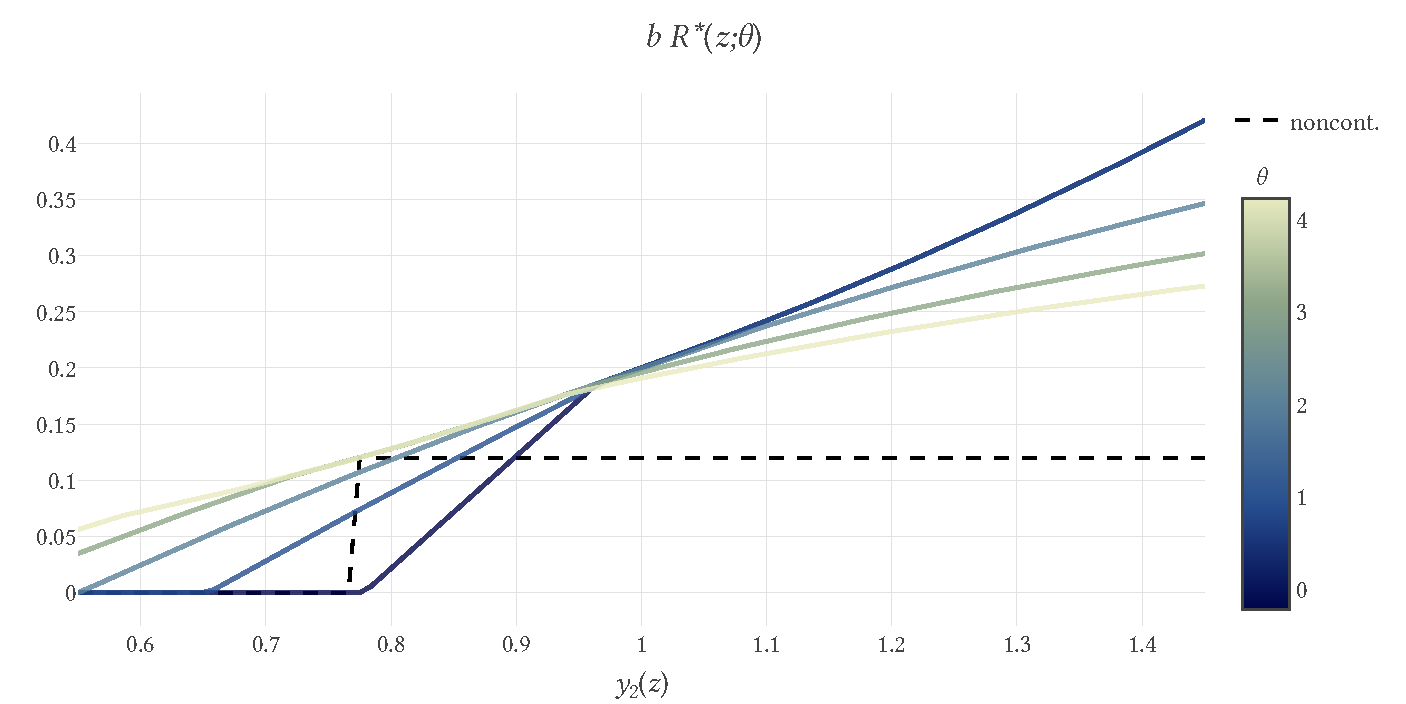
\includegraphics[width=0.9\textwidth]{arrow_paper.pdf}
\caption{Optimal design of state-contingent debt for each type of lender.
\label{Figure_arrow}}
\end{figure}
Figure \ref{Figure_arrow} sharply illustrates the tradeoffs in the debt-design problem when facing robust lenders. On the one hand, the government would like to minimize the contingency in stipulated repayments in order to prevent probability distortions. But the government also needs to minimize another source of contingency given by default risk ex-post. In low states, the government promises as much as it can credibly commit to repay.

\subsection{Spreads}\label{sec:spreads}
We now turn to how the probability distortions and concerns for model misspecification affect bond prices, issuances, and the government's welfare in equilibrium. The top panel of Figure \ref{Figure_spreads_parametric} shows our decomposition of equilibrium spreads as a function of the robustness parameter $\theta$. The bottom panel shows the issuance value $q(b)b$ as well as the welfare of the government. We measure welfare as the equivalent increase in consumption with respect to an equilibrium with the same $\theta$ but when the government issues noncontingent debt.\footnote{Somewhat abusing notation, if
\begin{align*}
  V(\theta, R, x) = u\left(c_1^b(1+x)\right) + \beta \mathbb{E}\left[u\left(c_2^b(1+x)\right)\right]
\end{align*}
is the value attained by the government, augmenting the equilibrium level of consumption by the factor $x$, then in each equilibrium with bonds $R$ and robustness $\theta$ we measure welfare by finding $x$ to make $V(\theta, R, 0) = V(\theta, 1, x)$.}
\begin{figure}[!hbtp]\centering
    \includegraphics[width=1\textwidth]{spreads_parametric_paper.pdf}
\caption{Spreads when the government issues the simple instruments. Bottom panel: issuance value $q(b)b$ and welfare difference from noncontingent debt}\label{Figure_spreads_parametric}
\end{figure}

When the government issues noncontingent debt, more robust lenders charge a higher spread for the ambiguity of default. The government responds by issuing lower amounts of debt. In our parametrization, the decrease in the default probability (the amount of risk) roughly compensates the increase in the spreads because of ambiguity (the price of risk).

Linearly-indexed debt successfully decreases the equilibrium default probability, as evidenced by lower spreads under rational-expectations. This leads to welfare gains equivalent to about $0.9\%$ of consumption from the noncontingent debt benchmark. As robustness increases, spreads from ambiguity of contingency and from ambiguity of default open up, eroding the government's ability to issue debt and therefore welfare gains. At $\theta = 4$, however, the government still values the option to move from noncontingent to linearly-indexed debt at about $0.8\%$ of consumption.

The picture is quite different for threshold debt. This type of debt completely eliminates default risk and therefore trades at no spreads with rational-expectations lenders. However, as $\theta$ increases, the large probability distortions discussed above support large spreads from the ambiguity of contingency. These high spreads quickly turn the welfare gains from state-contingent debt into welfare losses.

